\chapter{Diseño e implementación} % Main chapter title

\label{Chapter3} % Change X to a consecutive number; for referencing this chapter elsewhere, use \ref{ChapterX}

En este capítulo se abordará la descripción de la arquitectura general del sistema, la arquitectura del software, los módulos componentes del software, el desarrollo del software, el diseño del hardware, la selección y la calibración de sensores y el desarrollo de la aplicación movil.
\section{Diagrama de bloques}
En la figura \ref{fig:d_bloques} se muestra el diagrama en bloques general del sistema donde se describe la arquitectura aplicada al trabajo.

\begin{figure}[h]
\centering
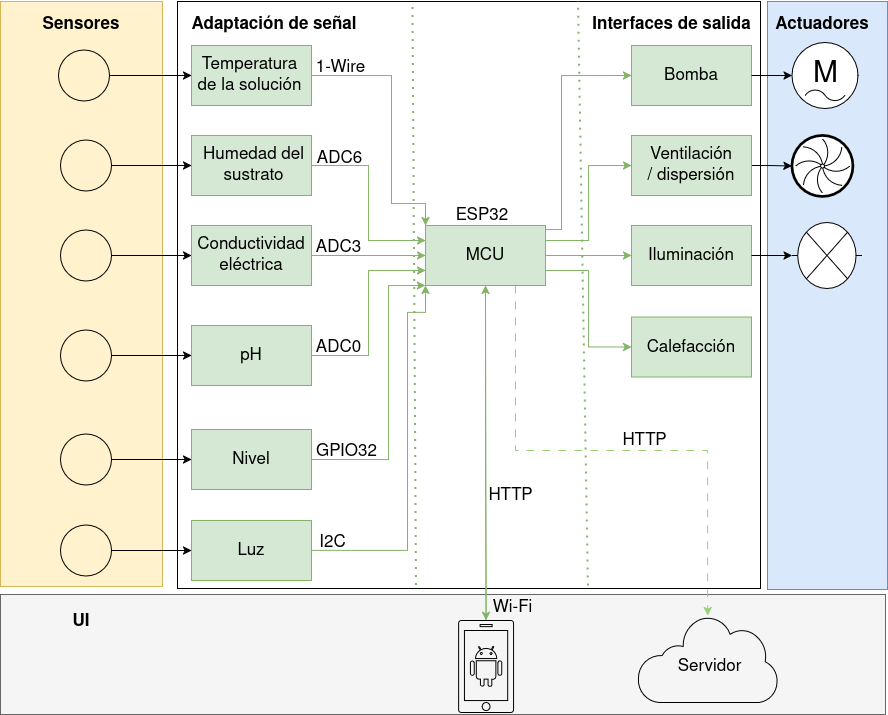
\includegraphics[scale=.4]{./Figures/d_bloques.png}
	\caption{Diagrama de bloques del sistema.}
	\label{fig:d_bloques}
\end{figure}

El sistema embebido implementado en este trabajo consta de una PCB centralizadora, diseñada para integrar y gestionar todos los módulos de hardware. Esta arquitectura asegura la alimentación, adaptación y protección de todos sus componentes. El sistema completo abarca desde la adquisición de datos mediante sensores hasta las acciones sobre el entorno a través de actuadores. Además, se complementa con una interfaz de usuario móvil para el monitoreo y control remoto.

A continuación, se describen brevemente los bloques y su función.

\begin{itemize}
	\item Sensores: este bloque se encarga de la transducción de magnitudes físicas en señales eléctricas, lo que permite la digitalización de variables ambientales de interés para el control del cultivo.
	\item Adaptación de señal: los módulos de adaptación acondicionan las señales provenientes de los sensores. Para garantizar la correcta interpretación por parte de la unidad de microcontrolador o MCU (del inglés \textit{MicroController Unit}), ajustan los niveles de tensión y la relación señal-ruido a valores apropiados.
	\item MCU: el núcleo del sistema, basado en el chip ESP32, orquesta la comunicación y el control de todos los módulos. Provee la capacidad de procesamiento y la conectividad inalámbrica necesarias para la automatización del cultivo y la interacción con la aplicación móvil.
	\item Interfaces de salida: proporciona aislamiento galvánico y acondicionamiento de potencia para la activación de los actuadores, lo que asegura la protección del MCU y la correcta operación de los componentes de mayor potencia.
	\item Actuadores: los actuadores (ventiladores, bomba de irrigación, luces, resistencia calefactora) ejecutan las acciones de control y modifican las condiciones ambientales del cultivo según las necesidades.
	\item Aplicación móvil de usuario: desarrollada para facilitar la interacción con el sistema, la aplicación móvil permite el monitoreo en tiempo real de las condiciones del cultivo y el control remoto de los actuadores.
	\item Interfaz de servicio web: se implementó una interfaz para la transmisión de datos a un servicio web externo que permite el almacenamiento y análisis de información del cultivo. Esta funcionalidad se encuentra fuera del alcance principal de este trabajo.

\end{itemize}

\section{Arquitectura del firmware}

En la presente sección se aborda la arquitectura del firmware del microcontrolador.

\subsection{Patrones}

A continuación, se detallan los patrones de diseño arquitectónico utilizados.

\subsubsection{Arquitectura en capas}
Se adoptó un patrón de arquitectura en capas para estructurar el software desarrollado, lo que permitió una separación de funcionalidades clara mediante niveles de abstracción. Dicha metodología divide el sistema en niveles horizontales, cada uno con responsabilidades específicas y bien definidas, que facilita el desarrollo, la mantenibilidad y la escalabilidad del código.

A continuación, se enumeran las capas de abstracción que constituyen el firmware.

\begin{itemize}
	\item Capa de aplicación.
	\item Capa de sistema operativo.
	\item Capa de abstracción de hardware (HAL).
\end{itemize}


\subsubsection{Capa de abstracción de hardware}

Para facilitar la interacción con los diversos componentes de hardware y garantizar la portabilidad del código, se implementó una capa de abstracción basada en Espressif HAL (\textit{Hardware Abstraction Layer}). Integrada dentro del SDK de ESP-IDF, esta capa proporciona una interfaz uniforme para el control de los periféricos del ESP32, independientemente de las particularidades del hardware subyacente.

\subsubsection{Control ambiental}

El patrón de control ambiental se adoptó como estrategia arquitectónica para la capa de aplicación. El sistema embebido requirió la monitorización y modificación del entorno mediante sensores y actuadores. Este patrón permitió la estructuración de la lógica de control y facilitó la gestión de las interacciones entre los componentes de hardware y la implementación de los algoritmos de control.


\subsection{Componentes}

La capa de aplicación, figura \ref{fig:arq_bloques}, está constituida por los componentes de software encargados de gestionar cada una de las funcionalidades del sistema.
A continuación, se describe brevemente la funcionalidad de cada uno de estos componentes.

\begin{itemize}
	\item Monitor de temperatura: mide la temperatura de la solución nutritiva para garantizar que las plantas crezcan en un entorno térmicamente adecuado.
	\item Monitor de conductividad eléctrica (CE): evalúa la concentración de nutrientes presentes en la solución hidropónica.
	\item Monitor de nivel: monitorea que el nivel de solución nutritiva en el sistema no caiga por debajo de un valor determinado.
	\item Monitor de pH: mide el nivel de acidez de la solución nutritiva, lo que ayuda a mantener el pH dentro del rango óptimo para el cultivo.
	\item Monitor de humedad del sustrato: mide el contenido de humedad en el sustrato del cultivo.
	\item Monitor de luz: mide la cantidad de luz disponible en el entorno a través de un sensor.
	\item Servidor web embebido: el servidor web embebido permite la comunicación con el sistema de control del cultivo a través de la red. Este servidor permite monitorear, configurar y controlar el sistema desde cualquier dispositivo con acceso a la red.
	\item Control de ciclo de luz: este módulo se encarga de gestionar el ciclo de iluminación del cultivo. La configuración de dicho ciclo se realiza por medio de la interfaz de usuario.
	\item Control de ciclo de oxigenación/ventilación: este componente activa y desactiva el flujo de aire en el sistema de cultivo según la configuración del usuario.
	\item Control de hidratación: gestiona el riego, activa la bomba de agua y ajusta los niveles de humedad del sustrato según las mediciones del sensor de humedad. Esto asegura la cantidad adecuada de agua para el desarrollo de las plantas.
	\item Administrador: es el componente encargado de la centralización y validación global de los datos suministrados por los demás módulos de software.
\end{itemize}



\begin{figure}[h]
\centering
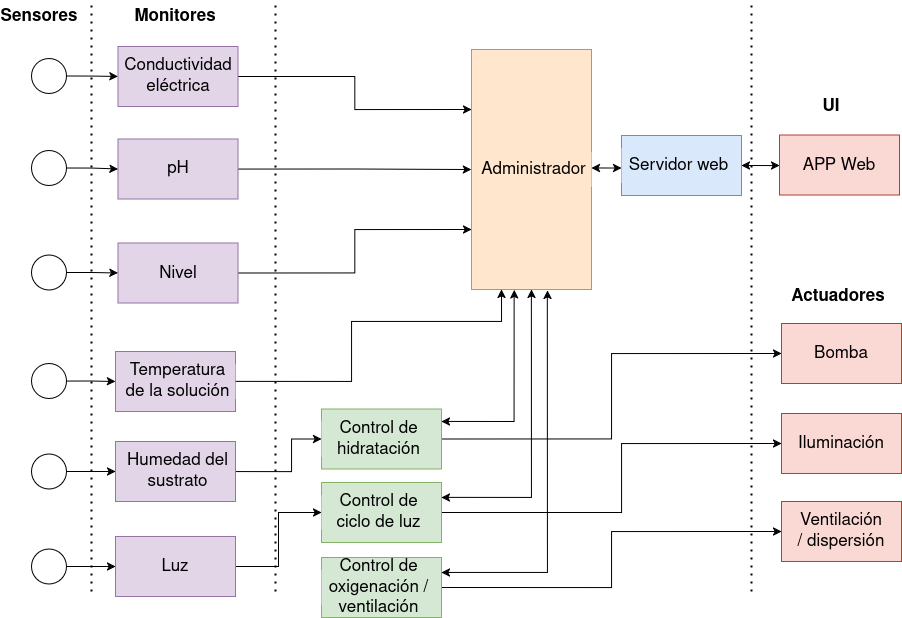
\includegraphics[scale=.4]{./Figures/arq_bloques.png}
	\caption{Diagrama de módulos funcionales y sus interacciones.}
	\label{fig:arq_bloques}
\end{figure}



\section{Desarrollo del software}

Para facilitar la escalabilidad de la aplicación, se implementó una tarea de FreeRTOS para cada componente del firmware. Esta arquitectura modular permite modificar cada componente de forma independiente, sin afectar al resto del sistema.

\subsection{Gestión de la comunicación entre tareas}
La comunicación entre tareas se gestiona mediante un patrón de publicación/suscripción con múltiples canales, que utiliza colas de FreeRTOS como buffers para el intercambio de datos. Esta arquitectura desacopla los productores de información (ej., monitores) de los consumidores (ej., controlador, administrador), lo que garantiza la integridad de los datos y la estabilidad del sistema al evitar condiciones de carrera.

\subsection{Gestión de la prioridad}
Durante el desarrollo del firmware, se abordó la organización de las tareas considerando el clásico problema de productores-consumidores. Esta estrategia permitió estructurar el sistema en función del flujo de información entre tareas.

Se definieron los monitores como tareas productoras, encargadas de obtener datos del entorno mediante sensores y publicarlos en estructuras compartidas .

Se implementaron los controladores como tareas consumidoras, cuya función es tomar decisiones en base a los datos recibidos y accionar los actuadores correspondientes.

Se desarrolló una tarea de administrador, también consumidora, responsable de coordinar el funcionamiento general del sistema y gestionar configuraciones.

El servidor embebido fue programado con un doble rol: responde a eventos generados por el usuario (como solicitudes de información o configuraciones) y también produce eventos que otras tareas consumen, como actualizaciones de parámetros.

Se asignaron diferentes niveles de prioridad a las tareas según su disponibilidad requerida. Las tareas de monitoreo se crearon con prioridad intermedia, mientras que las tareas de control y administración se configuraron con mayor prioridad para asegurar tiempos de respuesta adecuados ante eventos prioritarios. El servidor, al depender de la interacción del usuario, fue asignado con prioridad alta.

\subsection{Controladores de dispositivos}

Se desarrollaron controladores de dispositivos (\textit{device drivers}) dedicados a gestionar directamente las unidades de hardware involucradas en el sistema.

Estos controladores permiten abstraer las operaciones de bajo nivel necesarias para interactuar con sensores y actuadores.

\subsection{Gestión de fallos}
El sistema incorpora mecanismos de detección y manejo de fallos tanto a nivel de hardware como de software. Cada tarea cuenta con rutinas de supervisión que permiten identificar comportamientos anómalos o pérdida de respuesta de los dispositivos. En caso de error, se activan procedimientos de contingencia que buscan restablecer el funcionamiento sin comprometer la estabilidad del sistema general.

Por ejemplo, si un sensor deja de enviar datos válidos durante un tiempo determinado, se genera una alerta que es registrada y comunicada al usuario. De igual modo, si un actuador no responde a una orden tras múltiples intentos, se desactiva su uso y se notifica al sistema mediante una bandera de estado.

Además, se implementó un mecanismo de \textit{watchdog} que reinicia automáticamente el microcontrolador en caso de bloqueo o error crítico no recuperable. La configuración base del usuario se almacena en memoria no volátil (NVS), lo que permite que el sistema se recupere de cortes de energía sin perder los parámetros definidos.

\subsection{Servidor embebido}
Para facilitar la interacción con el usuario, el sistema cuenta con un servidor embebido basado en HTTP alojado en la propia ESP32. Este servidor permite exponer una API REST, a través de la cual se puede monitorear el estado del cultivo, consultar los valores de los sensores en tiempo real y ejecutar acciones como el encendido manual de actuadores o la configuración de alertas.

El servidor opera de forma concurrente con el resto de las tareas del sistema gracias a la arquitectura multitarea de FreeRTOS. Para garantizar la seguridad de acceso, se implementó un sistema básico de autenticación por usuario y contraseña que protege las rutas de la API.

El servidor responde a peticiones HTTP provenientes tanto de navegadores como de la aplicación móvil desarrollada en React Native, que primero transmite las credenciales de red por Bluetooth para iniciar la conexión Wi-Fi y luego se comunica mediante la API expuesta.

Este servidor embebido representa un componente clave para el monitoreo remoto y la escalabilidad del sistema, ya que permite una integración sencilla con otras plataformas IoT o bases de datos externas si se desea en el futuro.

\subsection{Lógica de negocio e interacción con la aplicación móvil}
La interacción entre la aplicación móvil y el dispositivo se desarrolla en dos etapas principales: configuración inicial por Bluetooth y comunicación operativa vía HTTP.

\subsubsection{Fase de configuración}
Al iniciar el sistema por primera vez o tras un reinicio de red, la aplicación móvil se conecta a la ESP32 mediante \textit{Bluetooth Low Energy} (BLE). A través de esta conexión, el usuario ingresa las credenciales de su red Wi-Fi doméstica (SSID y contraseña), que son transmitidas de forma segura al microcontrolador. Una vez recibidos estos datos, el dispositivo intenta conectarse a la red y, de ser exitoso, inicia el servidor embebido.

\subsubsection{Fase operativa}
Luego de establecer conexión Wi-Fi, la ESP32 expone una API REST que permite a la aplicación móvil interactuar con el sistema. Entre las operaciones más importantes se incluyen:

\begin{itemize}
	\item Lectura de datos ambientales (temperatura, humedad, pH, EC, etc.).
	\item Consulta del estado de los actuadores (iluminación, bomba, ventilación).
	\item Configuración de parámetros personalizados y umbrales de alerta.
	\item Activación manual o automática de funciones del sistema.
	\item Acceso a registros de eventos o errores del sistema.
\end{itemize}

\subsubsection{Manejo de estados y sincronización}
El firmware mantiene una estructura centralizada de datos en memoria que refleja el estado actual del sistema. Esta información se sincroniza con la app móvil cada vez que se establece una sesión HTTP válida. De este modo, el usuario siempre visualiza información actualizada del estado del cultivo.

Además, se contempló la posibilidad de incorporar una capa adicional de persistencia remota, como sincronización con bases de datos externas o servicios en la nube, lo que permitirá futuras extensiones del sistema hacia modelos más complejos de análisis de datos o inteligencia artificial.


